\documentclass{beamer}
\usetheme{Madrid}
\usecolortheme{default}

\usepackage[utf8]{inputenc}
\usepackage[T1]{fontenc}
\usepackage{amsmath}
\usepackage{algorithm}
\usepackage{algorithmic}
\usepackage{tikz}

\title{Maximum Number of Darts Inside of a Circular Dartboard}
\subtitle{LeetCode 1453}
\author{Nikola Labus}
\date{\today}

\begin{document}

\begin{frame}
\titlepage
\end{frame}

\begin{frame}{Sadržaj}
\tableofcontents
\end{frame}

\section{Problem}

\begin{frame}{Definicija problema}
\begin{block}{Problem}
Dato je $n$ strelica na zidu, gde je $\text{darts}[i] = (x_i, y_i)$, i poluprečnik $r$.\\[6pt]
Naći \textbf{maksimalan broj strelica} koje mogu biti unutar kružnog dartboard-a poluprečnika $r$.
\end{block}

\vspace{10pt}

\begin{block}{Ograničenja}
\begin{itemize}
    \item $1 \leq n \leq 100$
    \item $-10^4 \leq x_i, y_i \leq 10^4$
    \item $1 \leq r \leq 5000$
\end{itemize}
\end{block}
\end{frame}

\begin{frame}{Primeri}
\begin{columns}
\begin{column}{0.5\textwidth}
\textbf{Primer 1:}\\[4pt]
$\text{darts} = [(-2,0),(2,0),(0,2),(0,-2)]$\\
$r = 2$\\[4pt]
\textbf{Output: 4}\\[4pt]
Sve strelice su na krugu sa centrom u $(0,0)$.
\end{column}

\begin{column}{0.5\textwidth}
\begin{center}
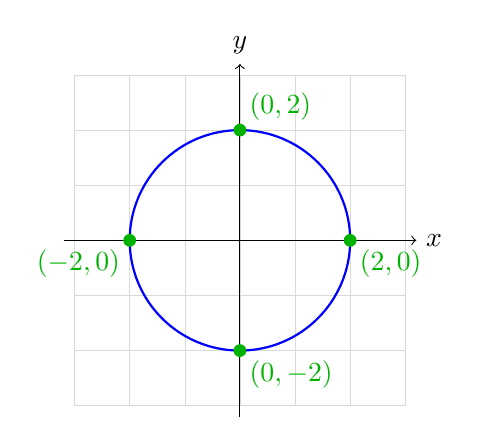
\begin{tikzpicture}[scale=0.7]
    \draw[help lines, gray!30] (-3,-3) grid (3,3);
    \draw[->] (-3.2,0) -- (3.2,0) node[right] {$x$};
    \draw[->] (0,-3.2) -- (0,3.2) node[above] {$y$};
    \draw[blue, thick] (0,0) circle (2);
    \filldraw[green!70!black] (-2,0) circle (3pt) node[below left] {$(-2,0)$};
    \filldraw[green!70!black] (2,0) circle (3pt) node[below right] {$(2,0)$};
    \filldraw[green!70!black] (0,2) circle (3pt) node[above right] {$(0,2)$};
    \filldraw[green!70!black] (0,-2) circle (3pt) node[below right] {$(0,-2)$};
\end{tikzpicture}
\end{center}
\end{column}
\end{columns}
\end{frame}

\section{Algoritam 1: Brute Force}

\begin{frame}{Ključna ideja}
\begin{block}{Observacija}
Optimalan krug \textbf{uvek prolazi kroz bar dve tačke} (ili jednu ako je $n=1$).
\end{block}

\vspace{10pt}

Zato je dovoljno isprobati sve parove tačaka i za svaki par naći moguće centre kruga poluprečnika $r$.

\vspace{10pt}

\begin{center}
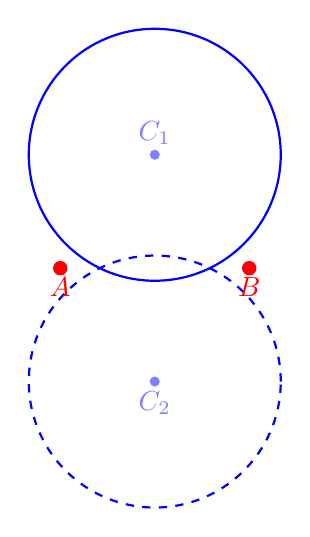
\begin{tikzpicture}[scale=0.8]
    \coordinate (A) at (-1.5, -0.5);
    \coordinate (B) at (1.5, -0.5);
    \draw[blue, thick] (0, 1.3) circle (2);
    \draw[blue, thick, dashed] (0, -2.3) circle (2);
    \filldraw[red] (A) circle (3pt) node[below] {$A$};
    \filldraw[red] (B) circle (3pt) node[below] {$B$};
    \filldraw[blue!50] (0, 1.3) circle (2pt) node[above] {$C_1$};
    \filldraw[blue!50] (0, -2.3) circle (2pt) node[below] {$C_2$};
\end{tikzpicture}
\end{center}
\end{frame}

\begin{frame}{Brute Force --- Pseudokod}
\begin{algorithmic}[1]
\FOR{svaki par tačaka $(i, j)$}
    \STATE Nađi rastojanje $d$ između njih
    \IF{$d > 2r$}
        \STATE Preskoči --- ne mogu biti na istom krugu
    \ENDIF
    \STATE Nađi dva moguća centra kruga koji prolazi kroz obe tačke
    \FOR{svaki centar}
        \STATE Prebroj koliko tačaka je unutar kruga
        \STATE Ažuriraj maksimum
    \ENDFOR
\ENDFOR
\end{algorithmic}
\end{frame}

\begin{frame}{Brute Force --- Složenost}
\begin{block}{Vremenska složenost}
\[
O(n^3)
\]
\begin{itemize}
    \item $O(n^2)$ parova tačaka
    \item Za svaki par: do 2 centra
    \item Za svaki centar: $O(n)$ provera
\end{itemize}
\end{block}
\end{frame}

\section{Algoritam 2: Angular Sweep}

\begin{frame}{Ideja Angular Sweep-a}
Umesto isprobavanja svih parova, za svaku tačku:

\begin{enumerate}
    \item \textbf{Fiksiraj} tačku $i$ na obod kruga
    \item \textbf{Rotiraj} krug oko tačke $i$
    \item Za svaku drugu tačku $j$, izračunaj \textbf{ugao ulaska} i \textbf{ugao izlaska} iz kruga
    \item \textbf{Sortiraj} događaje po uglu
    \item \textbf{Sweep}: prolazi po događajima i prati maksimalan count
\end{enumerate}

\vspace{10pt}

\begin{center}
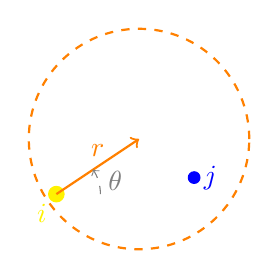
\begin{tikzpicture}[scale=0.7]
    \filldraw[yellow] (0,0) circle (4pt) node[below left] {$i$};
    \draw[orange, thick, dashed] (1.5, 1) circle (2);
    \draw[->, orange, thick] (0,0) -- (1.5, 1) node[midway, above] {$r$};
    \draw[gray, dashed, ->] (0.8,0) arc (0:34:0.8) node[midway, right] {$\theta$};
    \filldraw[blue] (2.5, 0.3) circle (3pt) node[right] {$j$};
\end{tikzpicture}
\end{center}
\end{frame}

\begin{frame}{Ugao ulaska i izlaska}
Za tačku $j$ u odnosu na pivot $i$:

\vspace{6pt}

\begin{align*}
d &= \text{dist}(i, j)\\[4pt]
\theta &= \text{atan2}(j_y - i_y,\ j_x - i_x) & \text{(ugao prema $j$)}\\[4pt]
\delta &= \arccos\left(\frac{d}{2r}\right) & \text{(polu-ugao)}
\end{align*}

\vspace{6pt}

\begin{block}{Događaji}
\begin{itemize}
    \item \textbf{Ulaz} na uglu $\theta - \delta$ \quad (count $+1$)
    \item \textbf{Izlaz} na uglu $\theta + \delta$ \quad (count $-1$)
\end{itemize}
\end{block}

\vspace{6pt}

Uslov: $d \leq 2r$ (inače tačka $j$ nikad ne ulazi u krug)
\end{frame}

\begin{frame}{Angular Sweep --- Pseudokod}
\begin{algorithmic}[1]
\FOR{svaku tačku $i$ (pivot)}
    \FOR{svaku drugu tačku $j$ na rastojanju $\leq 2r$}
        \STATE Izračunaj ugao ulaska i izlaska tačke $j$ iz kruga
        \STATE Zabeleži oba događaja
    \ENDFOR
    \STATE Sortiraj događaje po uglu
    \STATE Prolazi po događajima, prati count ($+1$ ulaz, $-1$ izlaz)
    \STATE Ažuriraj maksimum
\ENDFOR
\end{algorithmic}
\end{frame}

\begin{frame}{Angular Sweep --- Složenost}
\begin{block}{Vremenska složenost}
\[
O(n^2 \log n)
\]
\begin{itemize}
    \item $n$ tačaka (spoljašnja petlja)
    \item Za svaku: $O(n)$ događaja, sortiranje $O(n \log n)$
    \item Ukupno: $n \times O(n \log n) = O(n^2 \log n)$
\end{itemize}
\end{block}
\end{frame}

\section{Poređenje algoritama}

\begin{frame}{Poređenje}
\begin{center}
\begin{tabular}{|l|c|c|}
\hline
 & \textbf{Brute Force} & \textbf{Angular Sweep} \\
\hline
Vremenska složenost & $O(n^3)$ & $O(n^2 \log n)$ \\
\hline
Pristup & Svi parovi + centri & Rotacioni sweep \\
\hline
Prednost & Jednostavnost & Brzina \\
\hline
\end{tabular}
\end{center}

\vspace{10pt}

Za $n = 100$:
\begin{itemize}
    \item Brute Force: $\sim 10^6$ operacija
    \item Angular Sweep: $\sim 10^4 \cdot \log 100 \approx 6.6 \times 10^4$ operacija
\end{itemize}
\end{frame}

\begin{frame}{}
\begin{center}
\Huge Hvala na pažnji!

\vspace{20pt}

\large Pitanja?
\end{center}
\end{frame}

\end{document}
